% Chapter 2

\chapter{Background} % Main chapter title

\label{Chapter2} % For referencing the chapter elsewhere, use \ref{Chapter2} 

In this chapter, we will present some backgrounds on software attack and remote attestation to detect the attacks. After that, we will share an overview of LLVM that relevant to the research. 

\section{Software Attack}

Software attack happens when adversaries make program execution to perform action of their choice. The adversary choice can be executing malicious operations or leaking secret information and more. In the past adversary will modify the binary of the application to statically alter the the behaviour of the program. Nowadays, to prevent detection, attacks are being done by altering runtime properties of the program. Many of this runtime software security attacks are occured due to memory corruption bug in software written in low-level languages like C and C++ \cite{szekeresSoKEternalWar2013}.

Once memory corruption is triggered, there are different exploit types which adversary can use to perform the attack. Some of the relevant exploits are control-flow hijack \cite{shachamGeometryInnocentFlesh2007, schusterCounterfeitObjectorientedProgramming2015}  and data only attack \cite{chenNonControlDataAttacksAre2005, carliniControlFlowBendingEffectiveness2015}. Control-flow hijack can be classified further into code injection attack and code reuse attack such as return oriented programming \cite{roemerReturnorientedProgrammingSystems2012}. Code injection attack is already mitigated by Data Exectuion Prevention. A return-oriented program chains together short instruction sequences already present in a program’s address space, each of which ends in a “return” instruction. ROP can't be mititgated by \( W \bigoplus R \) or trusted computing

\section{Remote Attestation}
Remote attestation is the activity of making a claim about properties of a remote target by supplying evidence to an appraiser over a network \cite{cokerPrinciplesRemoteAttestation2011a}. The rampant deployment of IoT and different applications in the cloud require robust remote attestation method to ensure detection when the application is attacked.

Remote attestation scope was only covering static attestation of the application binary. However, in the recent years there have been more sophisticated attack that can alter the behavior of application so that static attestation will not suffice. 

In remote attestation there will be two roles involved, a trusted prover and a verifier. A prover is the one that must proof that the software hasn't been compromised. Verifier will check prover to ask the current state of runtime of the program. Alternatively, prover also can just update verifier periodically without being asked. The verifier will compare the response from prover with the local database which has been generated before. If any of measurement mismatches, it means the has been violation due to an adversary's attack.

This research will be mainly focused on offline measurement data generation for remote attestation which will be used by verifier to validate the control flow graph. We will be using LLVM in implementing the offline program analyzer.

\section{LLVM}

LLVM is compiler framework that was developed by Chris Lattner which provides portable program representation and different tooling. LLVM supports the implementation of different frontend, backend and middle optimizer for various programming languages \cite{lattnerLLVMCompilationFramework2004a}. 

\subsection{Intermediate Reprsentation}

LLVM intermediate representation (IR) provides high-level information about programs to support sophisticated analysis and transformations but low-level enough to represent arbitrary programs and to allow extensive optimization in it. As an example, consider a simple C program in listing \ref{listing:2-1}.

\begin{listing}
\inputminted[]{c}{code/sample.c}
\caption{Simple C Program}    
\label{listing:2-1}
\end{listing}

The IR of the program can be seen in listing \ref{listing:2-2}. The text representation below, is just one of form of IR. Beside this readable instruction representation, LLVM IR also can be represented as byte code and in memory representation.

\begin{listing}
\inputminted[]{llvm}{code/sample.ll}
\caption{LLVM IR The Sample C Program}    
\label{listing:2-2}
\end{listing}

In the IR, each line contains LLVM instructions. Instructions are grouped in basic blocks — container for instructions that execute sequentially. This arrangement, makes application control flow graph (CFG) to be explicit in the IR. From the C code and the IR above, the CFG graph is as follow.

\begin{figure}[htbp]
\centerline{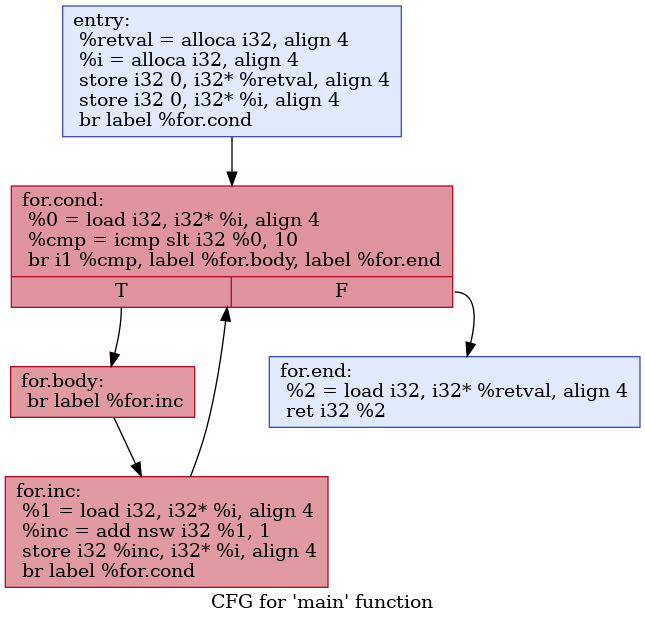
\includegraphics[scale=.5]{Figures/cfg.png}}
\caption{CFG for Simple C Program}
\label{fig:2-1}
\end{figure}

The details of LLVM IR is available in the Language Reference \cite{LLVMLanguageReferencea}.

LLVM optimizer — which includes Analyzer and Transformer — are working on IR. In this thesis we are using this analyzer and transformer in building the Offline Program Analyzer.

\subsection{LLVM Pass}

LLVM are applying transformations (which may include some analysis pipelines) and optimizations on tools called opt. opt is taking LLVM IR (either as text, bytecode or in memory) as input and then do transformations, analysis and optimizations on it. Transformation and optimization will alter the LLVM structure. Analysis will get information from the structure, which usually will be used by one or more transformations. Different transformations, optimizations and analyses are performed as pipelines of LLVM passes. LLVM pass can run per function, module or loop. LLVM function pass will be executed once for every function in the program. LLVM module pass will be executed once for every module. LLVM loop pass will run a time for each loop. 

\begin{figure}[htbp]
\centerline{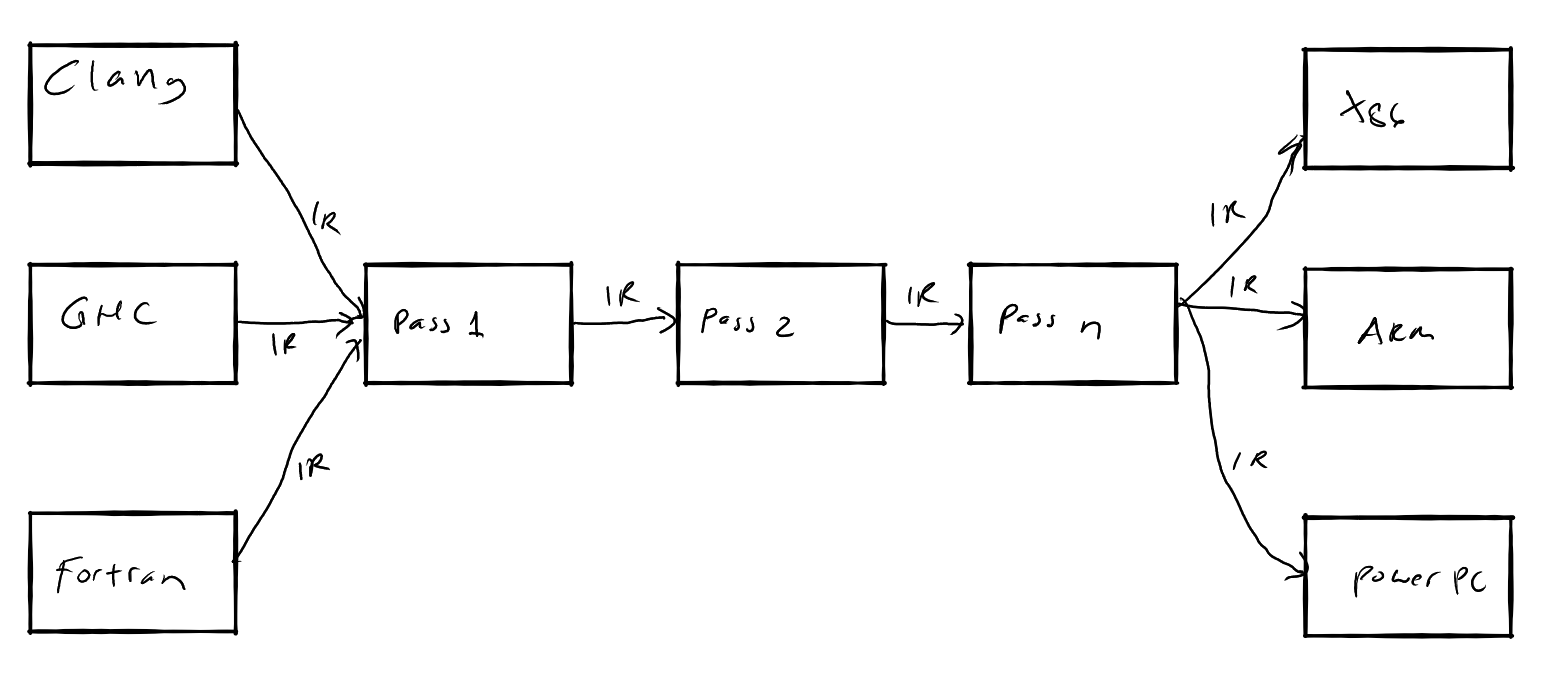
\includegraphics[scale=.25]{Figures/llvm.png}}
\caption{LLVM Pass (This is image will be replaced with the proper one)}
\label{fig:2-2}
\end{figure}

In LLVM there are two ways of implementing Pass. First is using legacy approach and the latest one is using new pass manager approach. The approach different in structuring the code the implement the pass and also the way we use the pass. 

In the legacy approach, we need to inherit from either ModulePass, FunctionPass or LoopPass and override runOnXXX method (xxx is either Function, Module or Loop). In the newer approach we have to inherit CRTP mix-in PassInfoMixin<PassT> and override the run method.

The way we use the pass, in legacy approach we need to provide the pass name as literal argument to opt. See the example below. In the new pass manager, we are putting the pass name after `--passes` argument in comma separated list. The pass will be executed in order.

\begin{listing}
\begin{minted}{bash}
    opt --dot-cfg file.ll 
\end{minted}
\caption{Running Legacy LLVM Pass}    
\label{listing:2-3}
\end{listing}

\begin{listing}
\begin{minted}{bash}
    opt -passes=scarr-cp-marker,scarr-loa-collector file.ll 
\end{minted}
\caption{Running LLVM New Pass}    
\label{listing:2-4}
\end{listing}

\subsection{LLVM API}

In writing LLVM pass, we will use LLVM API. In this section we will present relevant component that is required in implementing LLVM Pass for the Offline Program Analyzer. LLVM API is leveraging many C++ features and libraries such as template and STL. The API also provides many ready to use data structure which is not available in the STL. A more broad discussion on the important element of the API is available in the Programmers Manual \cite{LLVMProgrammerManuala}. Complete API documentation can be referred at the doxygen page \cite{LLVMLLVMa}.

\subsubsection{Module}

Module is the top level container for all other IR objects. Module contains list of global variables, functions, symbol tables and other various data about target characteristics. Module can be a single translation unit of a program (source file) or can be multiple translation unit combined by linker. 

In LLVM pass, we can get access to module by implementing a Module pass or by parsing IR using `parseIR` or `parseIRFile` from `IRReader.h`. Once we get a handler to a module, getting a functions within module will be as simple as passing module to a loop, since module provides iterator that return list of function in the module.

\begin{listing}
\inputminted[]{cpp}{code/module.cpp}
\caption{LLVM Module API}    
\label{listing:2-5}
\end{listing}

\subsubsection{Function}

Function in LLVM represents function in the source program. A function contains list of zero or more BasicBlocks. There will one entry BasicBlock and can be multiple exit BasicBlocks. We can get handler to a function either by getting the iterator from a module instance or by implement a Function Pass. By using optimization, syntax hint or using an inliner pass, a function can be inlined. In this thesis, we are using \emph{inliner-wrapper} pass to inline most function before feeding the IR into the ScaRR passes.

\subsubsection{Basic Block}

Basic Block represents single entry and single exit section of the code. The single exit can be one of terminator instruction — branches, return, unwind and invoke. We can get handle to a basic block from function. 

\begin{listing}
\begin{minted}{cpp}
    for (auto &function: *module) {
      for (auto &basicBlok: function) {
          // do thing with Basic Block
      }
    }
\end{minted}
\caption{LLVM Basic Block API}    
\label{listing:2-6}
\end{listing}

\subsubsection{Graph Traversal}

Since LLVM CFG is already structured as a graph, the basic block can be traversed using different ready to use graph traversal algorithm. LLVM offers some common graph traversal algorithms such as breadth first search and depth first search. The algorithms can be used immediately on basic blocks and functions. If there is a need to traverse a custom structure, the algorithms just require the new structure to implement \emph{GraphWriter} interface.

\subsection{Tools}

We are implementing the algorithms using different tools. We are highlighting some of those in this section so that everyone interested can replicate the step.

\subsubsection{clang}

clang is one of the frontend provided by LLVM. It can compiles C, C++ and Objective C. clang command line arguments are compatible with widely use gcc compiler. The main use of clang in this research is to compile source files into LLVM IR text files.

\begin{listing}
\begin{minted}{bash}
    clang -S -emit-llvm source.c
\end{minted}
\caption{Compiling C to LLVM IR}    
\label{listing:2-7}
\end{listing}
    
When compiling the source code, we can pass optimization level from 0 (no-optimization) to 3 (most optimal, can make code run faster but larger in size).  

By default, clang will strip out value names and do some optimization when generating LLVM IR. We can use this flag to disable optimization and get readable value names that can help when troubleshooting and exploring the generated IR.

\begin{listing}
\begin{minted}{bash}
    clang -S -emit-llvm -Xclang -disable-O0-optnone -fno-discard-value-names source.c
\end{minted}
\caption{Compiling C to LLVM IR without Optimization}    
\label{listing:2-8}
\end{listing}

\subsubsection{opt}

\emph{opt} is LLVM optimizer and analyzer that can be invoked from command line. We are using opt to execute the offline program analyzer which will mark basic block checkpoints and calculate list of action which can be used as information to detect control flow violation during remote attestation.

\subsubsection{cmake}

cmake is a build file generator which is have an important role in large project like LLVM. Although the deep understanding of cmake is not required in implementing LLVM pass, but we need to know at least how to build the pass after the implementation so that we can run it.

LLVM can be downloaded using git. This thesis is implemented on LLVM 13.0.0.

\begin{listing}
\begin{minted}{bash}
    git clone https://github.com/llvm/llvm-project
\end{minted}
\caption{Cloning LLVM Source Code}    
\label{listing:2-9}
\end{listing}

Once it is downloaded we can go to the LLVM directory and generate the build files. cmake supports several build tools such as make and ninja. 

\begin{listing}
\begin{minted}{bash}
    cd llvm-project/llvm
    mkdir build
    cd build
    cmake -G Ninja ../ # generate build file for Ninja
    ninja opt # build only opt
\end{minted}
\caption{Building LLVM}    
\label{listing:2-10}
\end{listing}